\begin{frame}[t]{Transporte de fluidos fica visível}
  \vspace{-0.35em}
  \begin{columns}[T,onlytextwidth]
    \column{0.60\textwidth}
      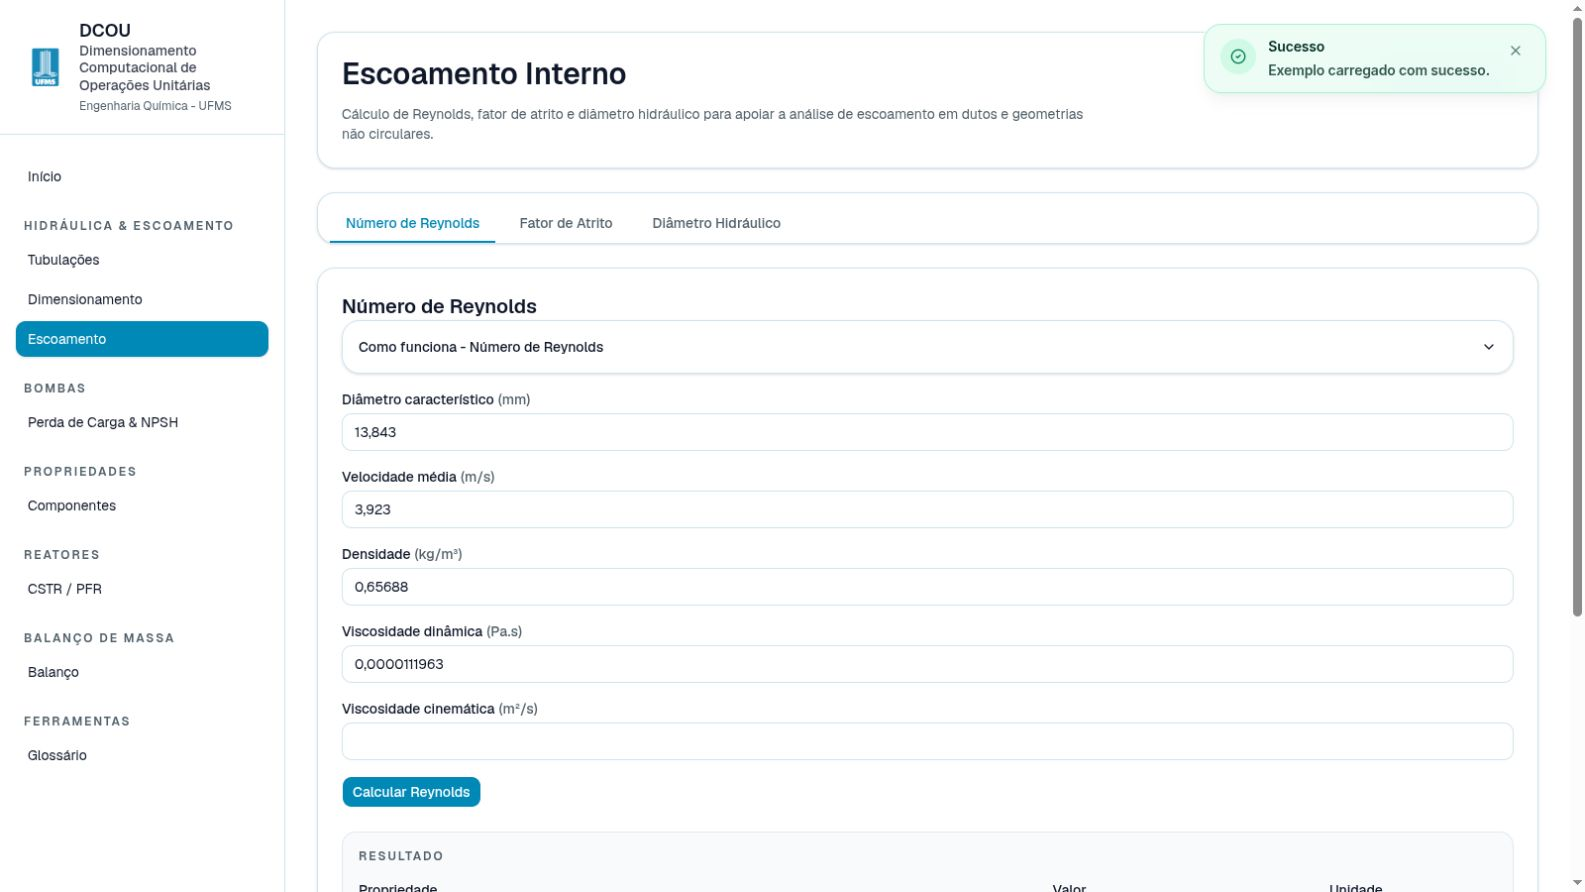
\includegraphics[width=\linewidth,height=0.56\textheight,keepaspectratio]{assets/screenshots/validated-flow-reynolds.png}
    \column{0.36\textwidth}
      \begin{block}{Inputs}
        \footnotesize
        \begin{itemize}
          \setlength{\itemsep}{0.18em}
          \item Diâmetro característico.
          \item Velocidade média.
          \item Densidade e viscosidade do fluido.
        \end{itemize}
      \end{block}
      \begin{block}{Outputs}
        \footnotesize
        \begin{itemize}
          \setlength{\itemsep}{0.18em}
          \item Número de Reynolds.
          \item Regime de escoamento.
          \item Leitura imediata do risco de transição.
        \end{itemize}
      \end{block}
  \end{columns}
\end{frame}

\begin{frame}[t]{Bombas conectam perda de carga e operação}
  \vspace{-0.35em}
  \begin{columns}[T,onlytextwidth]
    \column{0.60\textwidth}
      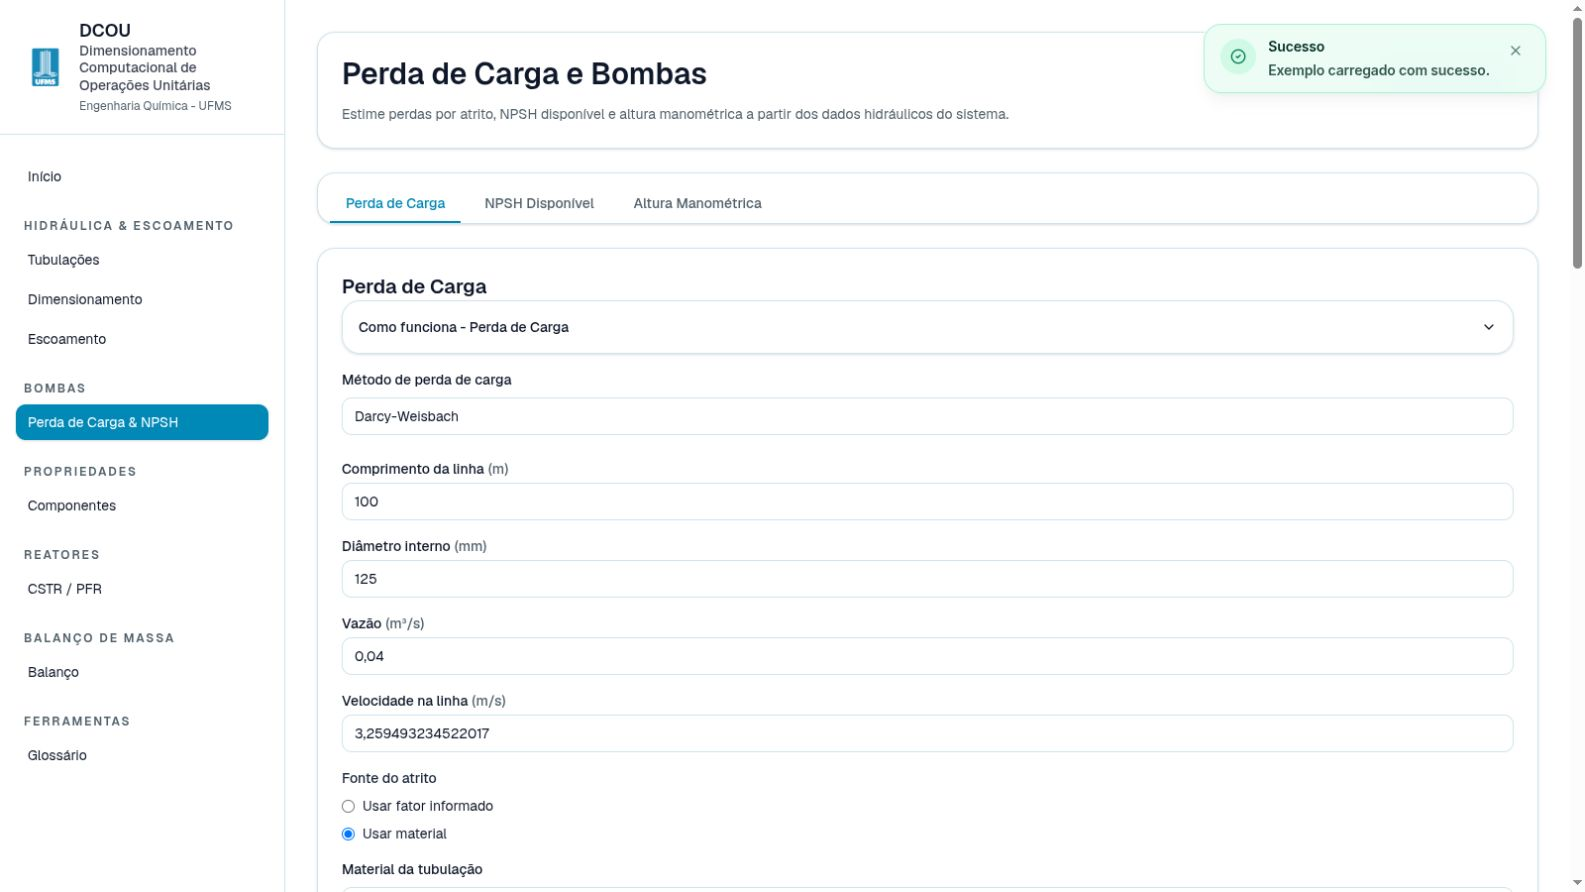
\includegraphics[width=\linewidth,height=0.56\textheight,keepaspectratio]{assets/screenshots/validated-pump-headloss.png}
    \column{0.36\textwidth}
      \begin{block}{Inputs}
        \footnotesize
        \begin{itemize}
          \setlength{\itemsep}{0.18em}
          \item Comprimento e diâmetro da linha.
          \item Vazão e velocidade.
          \item Método de atrito e condição de sucção.
        \end{itemize}
      \end{block}
      \begin{block}{Outputs}
        \footnotesize
        \begin{itemize}
          \setlength{\itemsep}{0.18em}
          \item Perda de carga calculada.
          \item NPSH disponível.
          \item Altura manométrica e faixa de operação.
        \end{itemize}
      \end{block}
  \end{columns}
\end{frame}

\begin{frame}[t]{Propriedades deixam de ser só tabela}
  \vspace{-0.35em}
  \begin{columns}[T,onlytextwidth]
    \column{0.60\textwidth}
      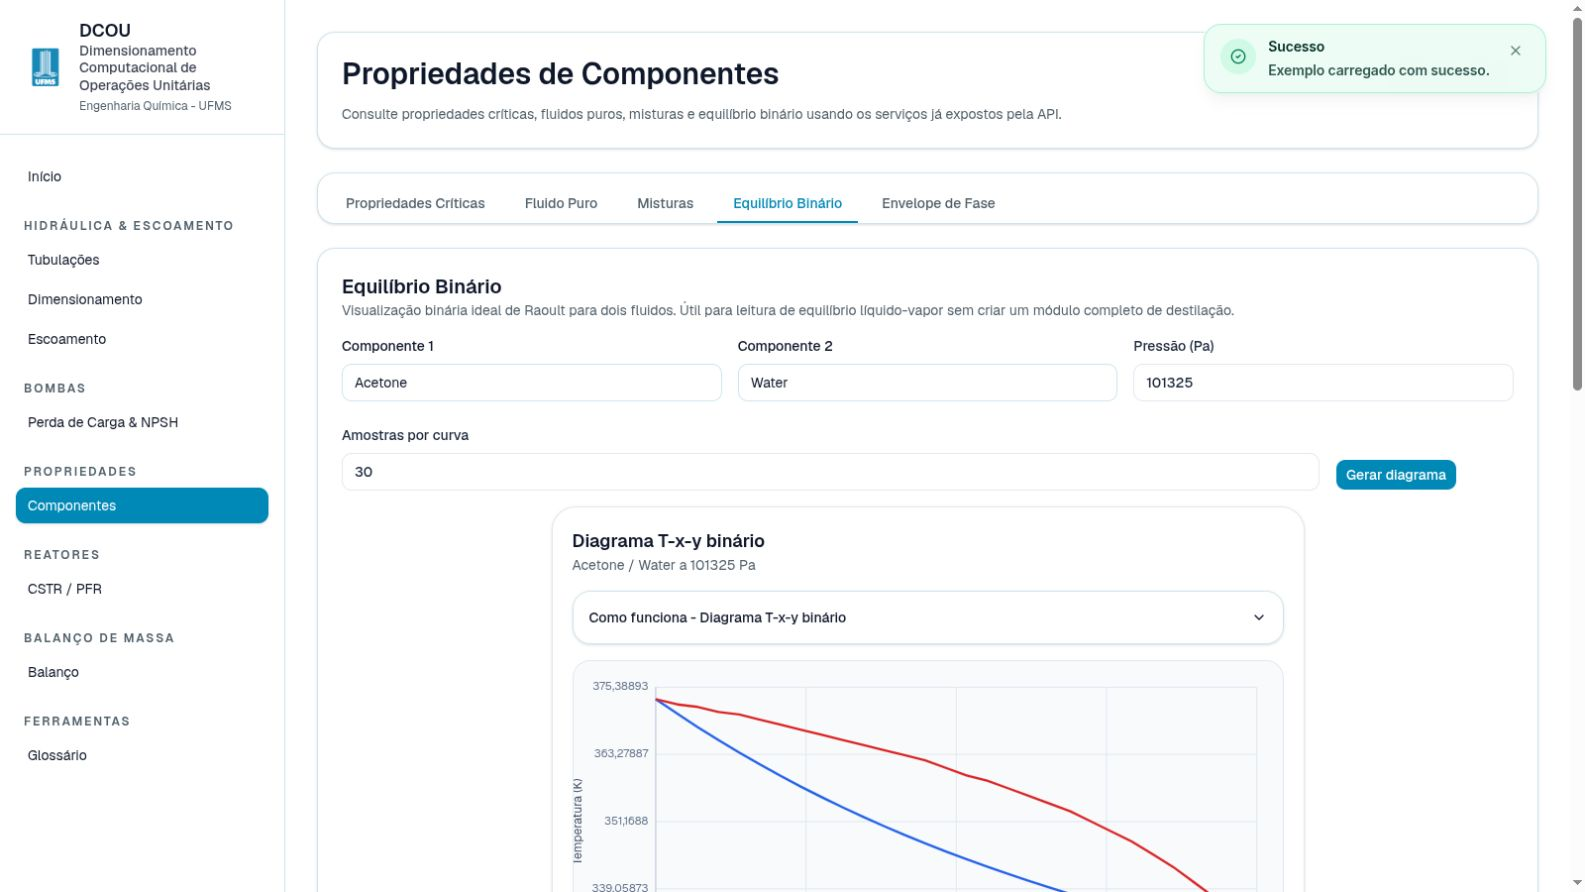
\includegraphics[width=\linewidth,height=0.56\textheight,keepaspectratio]{assets/screenshots/validated-components-binary-vle.png}
    \column{0.36\textwidth}
      \begin{block}{Inputs}
        \footnotesize
        \begin{itemize}
          \setlength{\itemsep}{0.18em}
          \item Dois componentes.
          \item Pressão de trabalho.
          \item Número de amostras da curva.
        \end{itemize}
      \end{block}
      \begin{block}{Outputs}
        \footnotesize
        \begin{itemize}
          \setlength{\itemsep}{0.18em}
          \item Diagrama T-x-y.
          \item Leitura de equilíbrio líquido-vapor.
          \item Suporte ao McCabe-Thiele e à separação.
        \end{itemize}
      \end{block}
  \end{columns}
\end{frame}

\begin{frame}[t]{Reatores fecham a cinética}
  \vspace{-0.35em}
  \begin{columns}[T,onlytextwidth]
    \column{0.60\textwidth}
      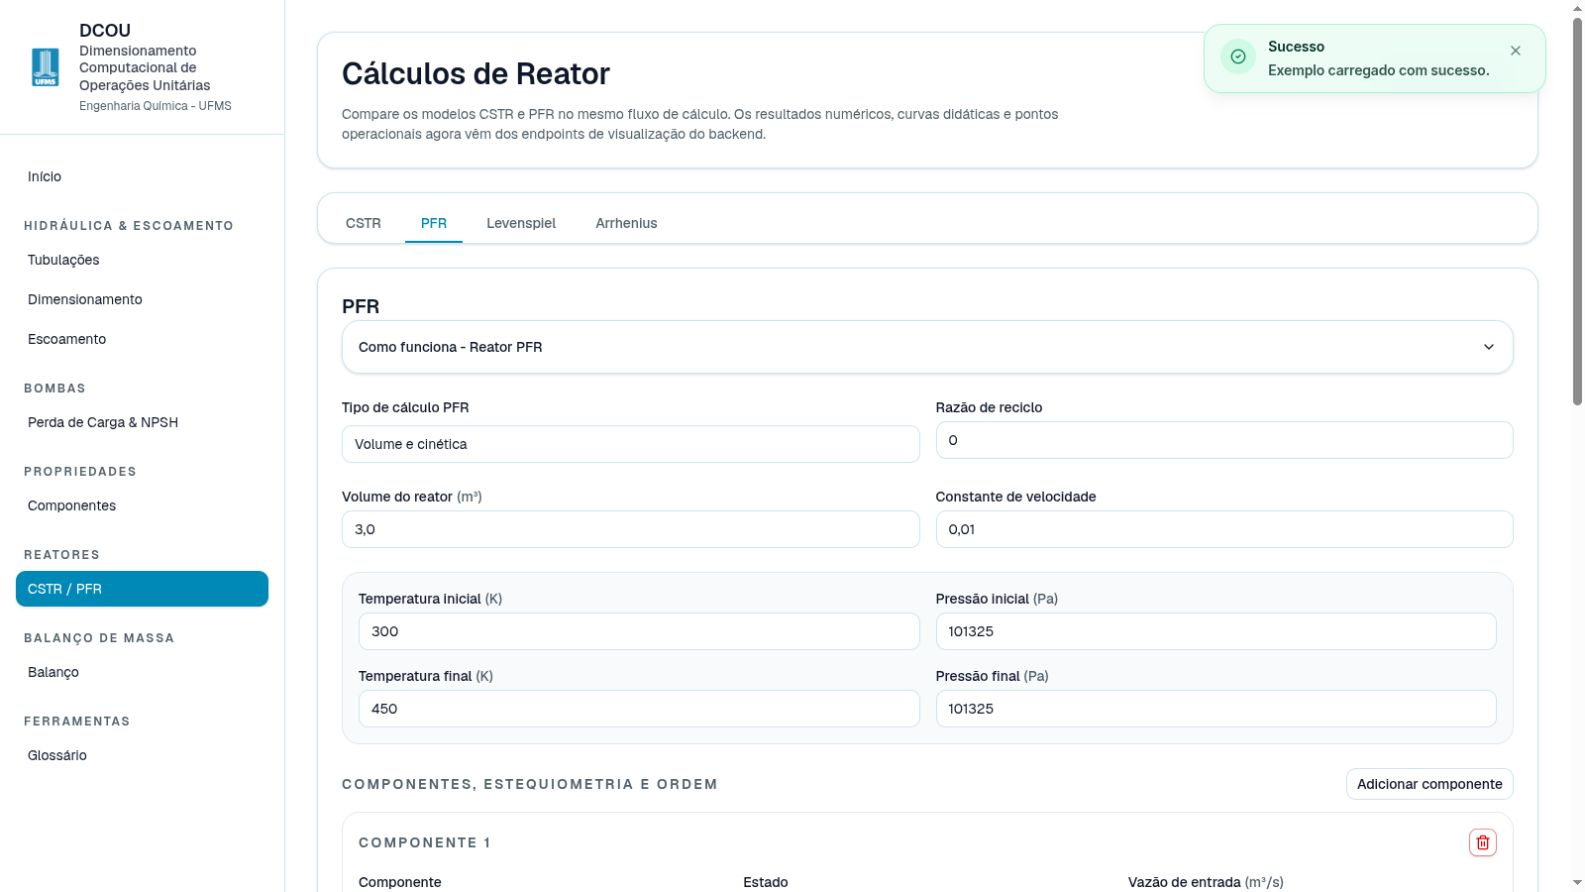
\includegraphics[width=\linewidth,height=0.56\textheight,keepaspectratio]{assets/screenshots/validated-reactor-pfr.png}
    \column{0.36\textwidth}
      \begin{block}{Inputs}
        \footnotesize
        \begin{itemize}
          \setlength{\itemsep}{0.18em}
          \item Volume do reator.
          \item Cinética e ordem de reação.
          \item Condições iniciais de operação.
        \end{itemize}
      \end{block}
      \begin{block}{Outputs}
        \footnotesize
        \begin{itemize}
          \setlength{\itemsep}{0.18em}
          \item Conversão calculada.
          \item Tempo de residência.
          \item Perfis e leitura operacional.
        \end{itemize}
      \end{block}
  \end{columns}
\end{frame}

\begin{frame}[t]{Balanço de massa fecha a matéria}
  \vspace{-0.35em}
  \begin{columns}[T,onlytextwidth]
    \column{0.60\textwidth}
      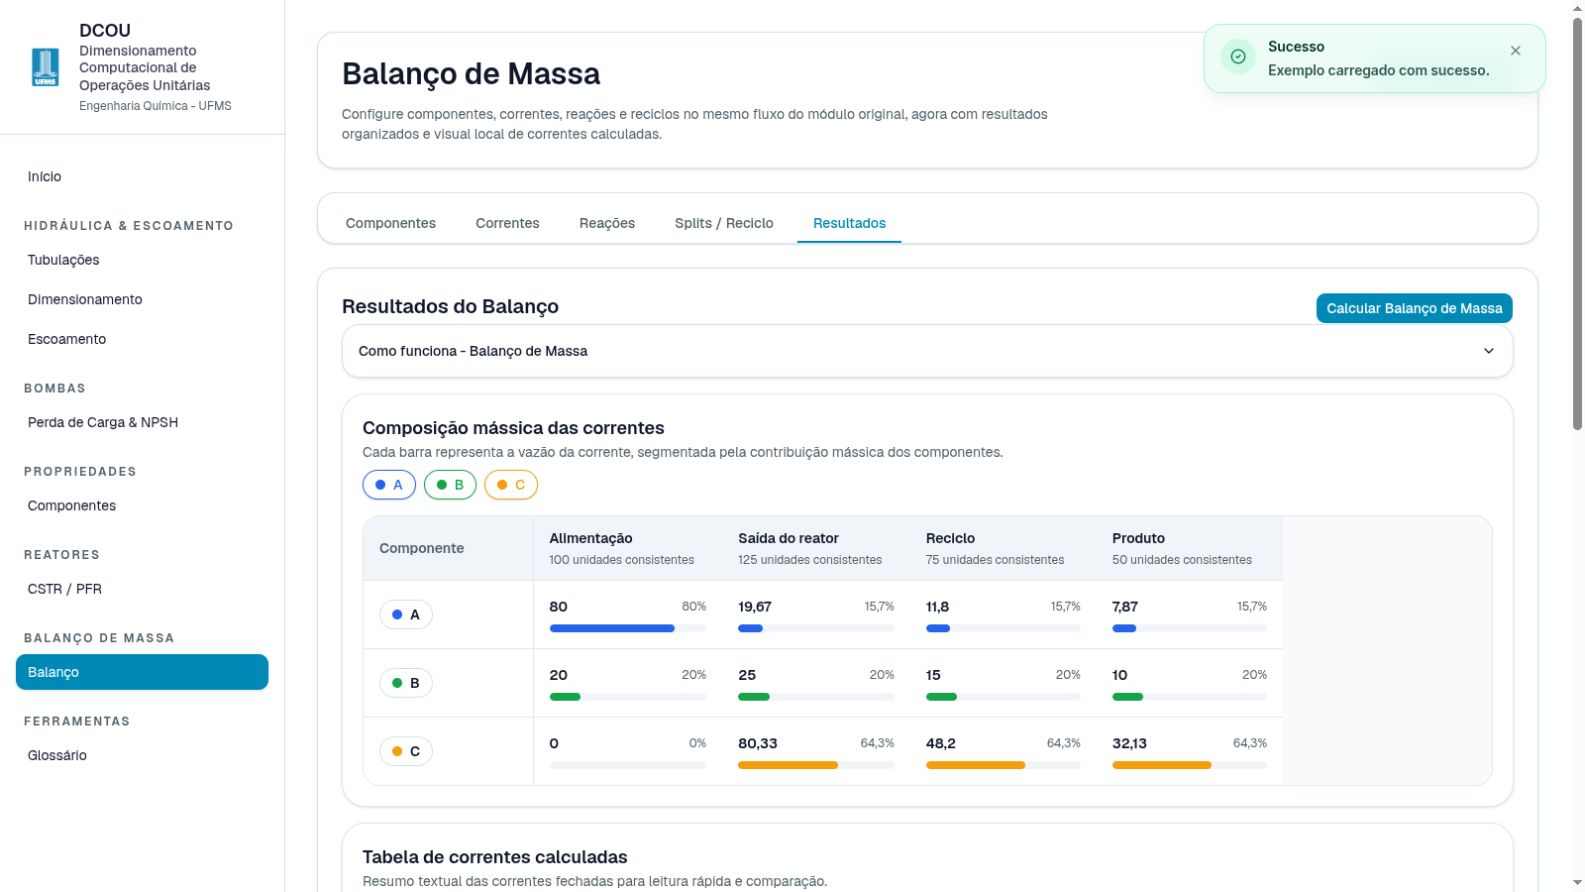
\includegraphics[width=\linewidth,height=0.56\textheight,keepaspectratio]{assets/screenshots/validated-balance-results.png}
    \column{0.36\textwidth}
      \begin{block}{Inputs}
        \footnotesize
        \begin{itemize}
          \setlength{\itemsep}{0.18em}
          \item Componentes da mistura.
          \item Correntes de entrada e saída.
          \item Reações e reciclo.
        \end{itemize}
      \end{block}
      \begin{block}{Outputs}
        \footnotesize
        \begin{itemize}
          \setlength{\itemsep}{0.18em}
          \item Correntes fechadas.
          \item Composição calculada.
          \item Leitura gráfica do balanço.
        \end{itemize}
      \end{block}
  \end{columns}
\end{frame}
